\section{Rectification}

The objective of this section is to establish a rectification mapping for the horizontal plane analyzed earlier and subsequently compute the object's depth. 
This process employs a stratified approach, beginning with Euclidean rectification followed by metric rectification.

\subsection{Euclidean rectification}
From geometric theory, the line at infinity identified in the previous step must be mapped to the real line at infinity in the scene.
Specifically, the line $\mathbf{l}^\prime_{\infty}$ in the image must be transformed back to $\mathbf{l}_{\infty}$: 
\[\mathbf{l}^\prime_{\infty}=\begin{bmatrix}
    a \\ b \\ c
\end{bmatrix}\xrightarrow[]{\text{mapped back to}}\begin{bmatrix}
    0 \\ 0 \\ 1
\end{bmatrix}=\mathbf{l}_{\infty}\]
To achieve this, we construct a homography matrix that aligns the line $\mathbf{l}^\prime_{\infty}$ with $\mathbf{l}_{\infty}$: 
\[\mathbf{H}_{\text{rect}}=\begin{bmatrix}
    1 & 0 & 0 \\
    0 & 1 & 0 \\
    a & b & c
\end{bmatrix}\]
By applying this transformation matrix to all pixels in the image, we obtain a rectified version of the scene. 
The resulting image is shown below:
\begin{figure}[H]
    \centering
    \includegraphics[width=0.75\linewidth]{images/rectified.jpg}
    \caption{Euclidean rectification}
\end{figure}

\subsection{Metric rectification}
Using a stratified approach, we proceed with the metric rectification step. 
This involves imposing orthogonality constraints to achieve a full metric reconstruction of the image.

We start by selecting two pairs of orthogonal lines: one pair along the lower side of the object and another pair intersecting near the top (ensuring the pairs are independent). 

From the selected pairs of lines $\mathbf{l}$ and $\mathbf{m}$, we compute the orthogonality conditions and populate a matrix $\mathbf{A}$.
Each row of $\mathbf{A}$ corresponds to the constraints imposed by one pair of lines, computed as follows:
\[\mathbf{A} = \begin{bmatrix} \mathbf{l}_x \cdot \mathbf{m}_x & \mathbf{l}_x \cdot \mathbf{m}_y + \mathbf{l}_y \cdot \mathbf{m}_x & \mathbf{l}_y \cdot \mathbf{m}_y \\ \cdots & \cdots & \cdots\end{bmatrix}\]
After constructing $\mathbf{A}$ using the selected two pairs of lines, we apply Singular Value Decomposition (SVD) to it.
The last row of the resulting $\mathbf{V}$ matrix contains the coefficients for the conic matrix $\mathbf{S}$, which is expressed as:
\[\mathbf{S}=\begin{bmatrix}
    \mathbf{V}(1,3) & \mathbf{V}(2,3) \\ \mathbf{V}(2,3) & \mathbf{V}(3,3)
\end{bmatrix}\]
To compute the homography matrix, we first find the transformation matrix $\mathbf{G}$, which is computed as
\[\mathbf{A}= \mathbf{U}\sqrt{\mathbf{D}}\mathbf{V}^T\]
Here, $\mathbf{U}$, $\mathbf{D}$, and $\mathbf{V}$ are obtained by performing Singular Value Decomposition on $\mathbf{S}$. 

The final metric rectification homography matrix is then given by:
\[\mathbf{H}_{\text{metric}}=\begin{bmatrix}
    \mathbf{G} & \mathbf{0} \\
    \mathbf{0} & 0
\end{bmatrix}\]
Applying $\mathbf{H}_{\text{metric}}$ to the rectified image transforms it into a fully metric rectified image. 
The resulting image is shown below:
\begin{figure}[H]
    \centering
    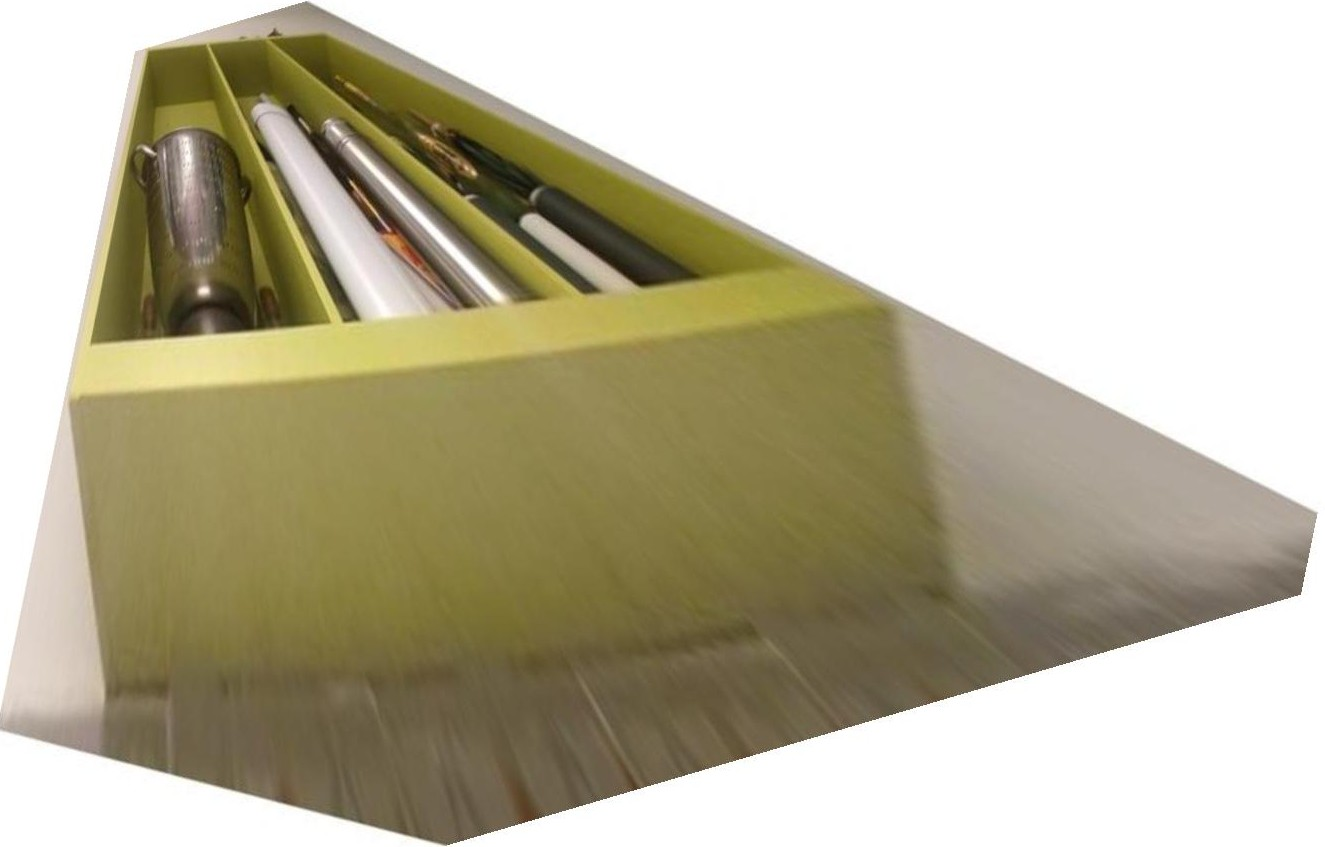
\includegraphics[width=0.75\linewidth]{images/metric.jpg}
    \caption{Metric rectification}
\end{figure}

\subsection{Depth computation}
The final step is to compute the object's depth using the metric rectified image. 
Assuming the object's width is known and unitary, we can measure both the width and depth directly on the rectified image using Euclidean distances between corresponding points.

The real-world depth is calculated as:
\[\text{real depth}=\dfrac{\text{depth}}{\text{width}} \cdot 1\]
This computation provides the actual depth of the object in proportion to its known width.